% ===================================================
% STCQ : Spatio-Temporal Collaboration Questionnaire
%
% Academic Reference:
% Nico Reski, Aris Alissandrakis, and Andreas Kerren. An Empirical Evaluation of Asymmetric Synchronous Collaboration Combining Immersive and Non-Immersive Interfaces Within the Context of Immersive Analytics. *Frontiers in Virtual Reality*, 2:743445:1-743445:29, January 2022. DOI: [10.3389/frvir.2021.743445](https://doi.org/10.3389/frvir.2021.743445)
%
% GitHub Repository:
% https://github.com/nicoversity/stcq
% 
% Repository Maintenance: Nico Reski
% Web: http://reski.nicoversity.com
% Twitter: @nicoversity
%
% ===================================================


\documentclass[10pt, onecolumn]{article}

% === PREAMBLE ===

\usepackage[utf8]{inputenc} 	% international symbols (incl. ä, ö, ü u.a.)
\usepackage[T1]{fontenc}		% international typeset
\usepackage[pdftex]{graphicx}	% use graphics
\usepackage[a4paper, top=10mm, left=15mm, right=15mm, bottom=18mm]{geometry}	% enabgle geometry functionality, A4 format
\usepackage{setspace}			% enable interleaf functionality
\usepackage[pdftex]{hyperref}	% enable hyperlinking
\usepackage{amssymb}            % mathematical signs
\usepackage{xcolor}             % enable color usage

\setstretch{1.3}				% set line height to be 130 %


% === DOCUMENT - START ===
\begin{document}


% === QUESTIONNAIRE HEADER ===
\begin{center}
    % GLADLY INSERT HERE THE TITLE OF YOUR INVESTIGATION
    {\Large \textbf{An Empirical Evaluation of a Collaborative HCI System\\     
    \vspace{\baselineskip}
    Spatio-Temporal Collaboration Questionnaire (STCQ)}}
\end{center}

\noindent
\textbf{Instructions}: For each of the following dimensions \textbf{[TSIA, NC, SC, AO]}, read carefully its definition, and for the questions / statements, mark \underline{\emph{one}} box that best describes your reactions to the tested application / interface.


\vspace{\baselineskip}
\noindent
{\large \textbf{Application / Interface}}   \hspace{38mm} {\large \textbf{Session}} 

% BASED ON YOUR SYSTEM DESIGN AND STUDY METHODOLOGY: GLADLY INSERT HERE THE NAMES / COMPONENTS / INTERFACES OF THE COLLABORATIVE SYSTEM AS OPERATED THROUGH THE INDIVIDUAL USERS, AS WELL AS THE TASK THEY COMPLETED (IN CASE OF MULTIPLE ONES)
\begin{tabular}{p{0.5cm}p{6cm}}
    $\square$   & Application / Interface X.\\
    $\square$   & Application / Interface Y.\\
\end{tabular}
\hspace{10mm}
%\hspace{80mm}
\begin{tabular}{p{2cm}p{6cm}}
    Date/Time:   & \rule{6cm}{0.5pt}\\
    Task:        & $\square$ 1 \hspace{0.2cm} $\square$ 2 \\
\end{tabular}


\vspace{\baselineskip}
\noindent\makebox[\linewidth]{\rule{\columnwidth}{0.4pt}}


% === QUESTIONNAIRE DIMENSIONS / ITEMS (PAGE 1) ===
\noindent
\textbf{[TSIA] Transitions between Shared and Individual Activities}: The interplay between individual and group efforts, including the ability to switch between these, within the scope of collaborative work.

\noindent
\begin{tabular}{p{1cm}p{9cm}p{8cm}}
TSIA.1  & How many of your efforts during this task would you consider to have been \emph{individual} efforts? 
    & \raisebox{-.5\height}{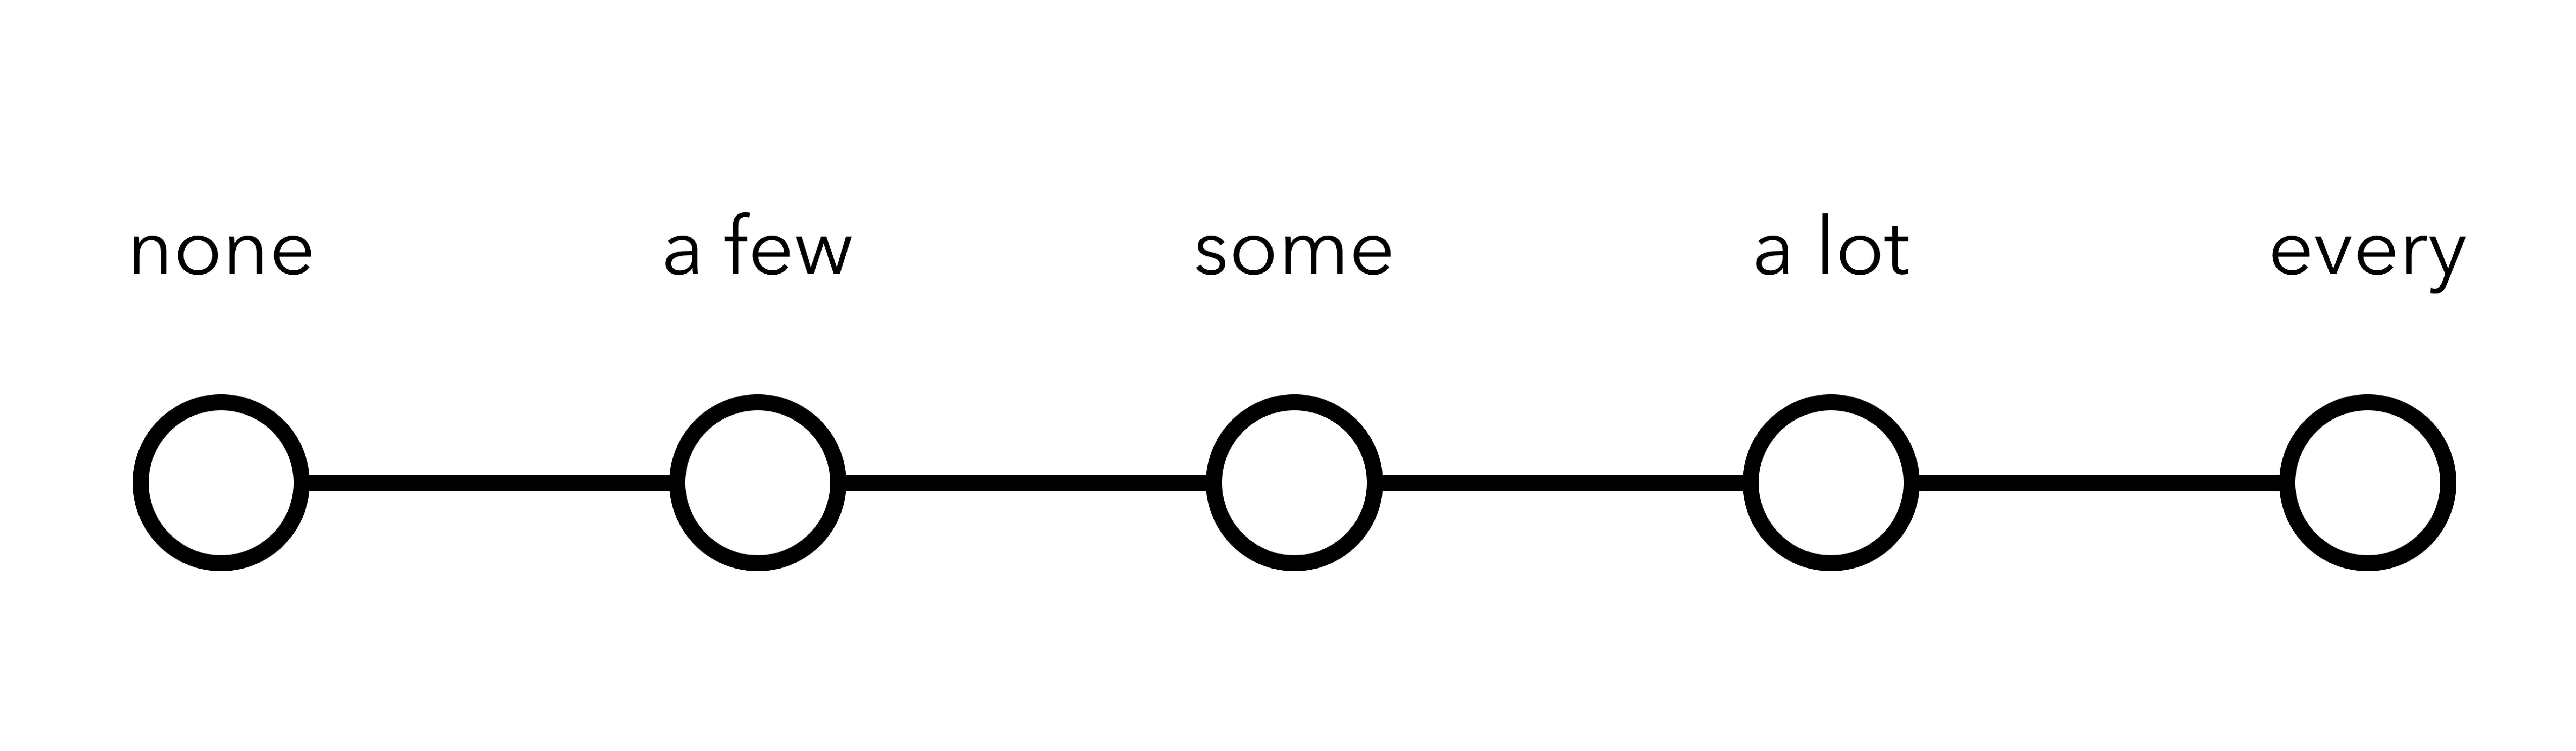
\includegraphics[width=7cm]{likert_scales/ls_5p-none_every}} \\
TSIA.2  & How many of your efforts during this task would you consider to have been \emph{group} efforts? 
    & \raisebox{-.5\height}{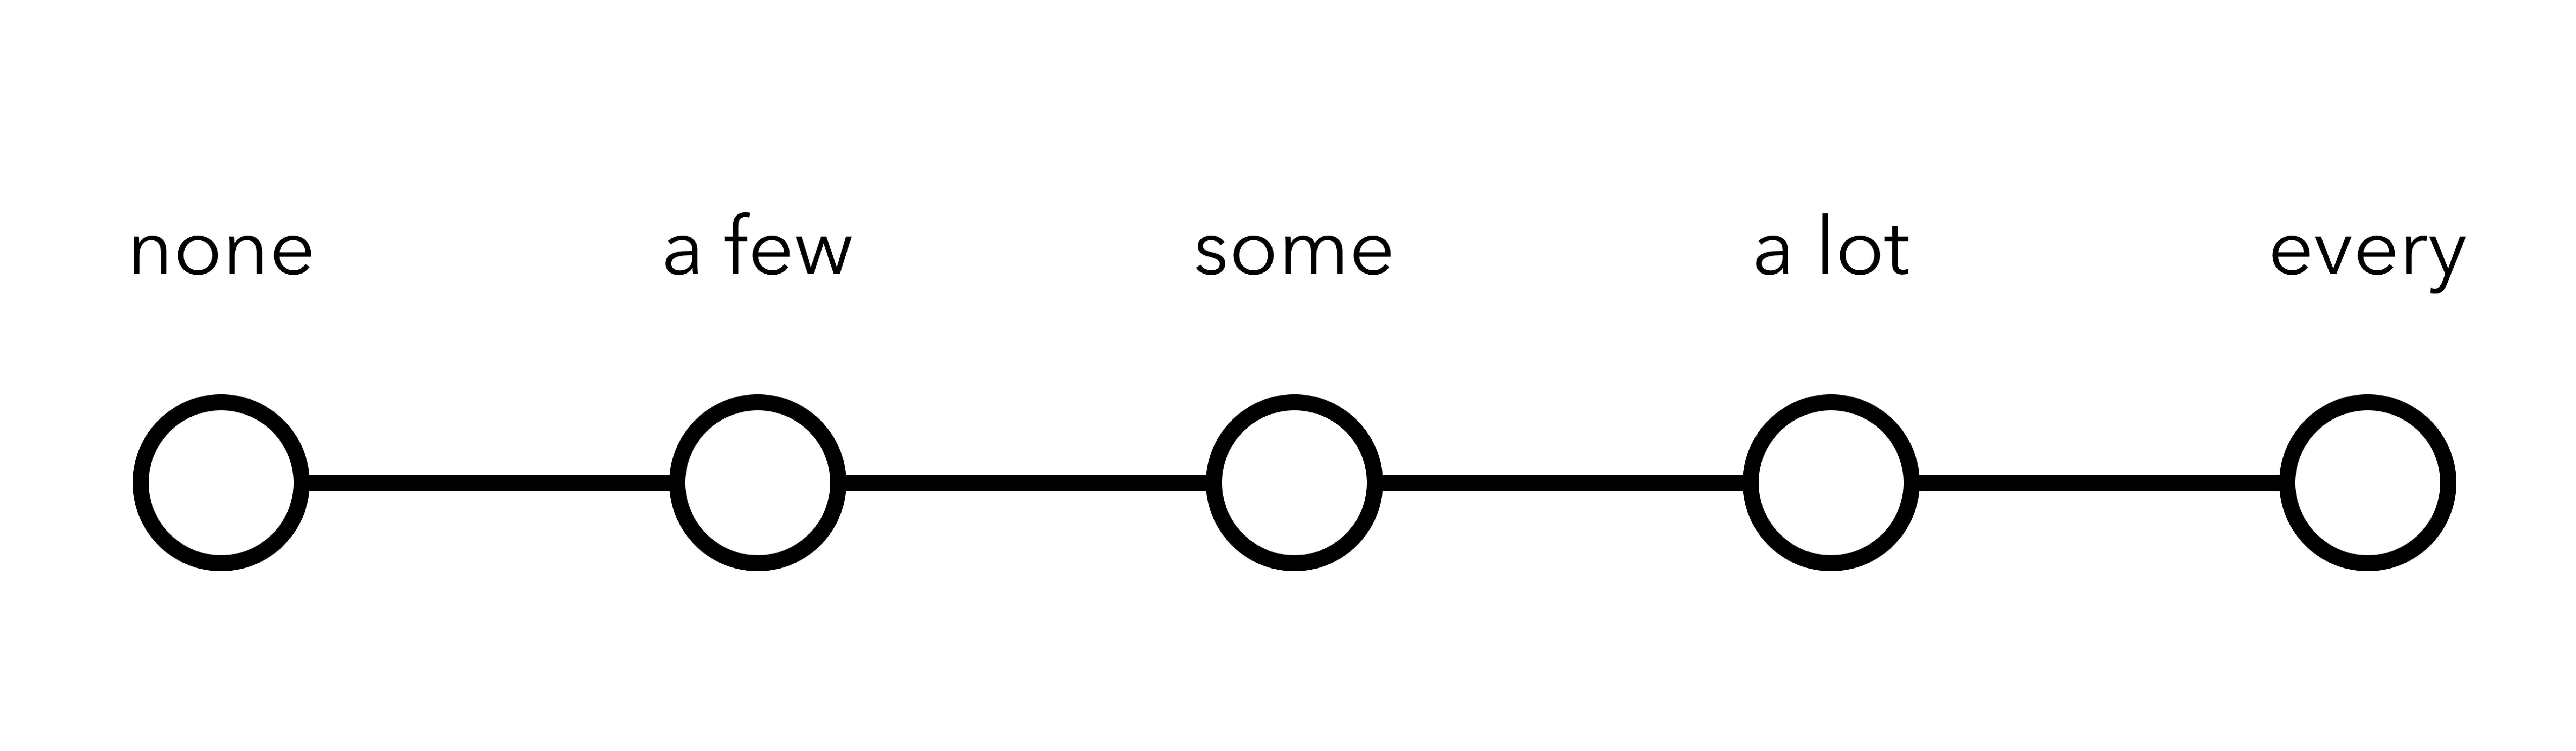
\includegraphics[width=7cm]{likert_scales/ls_5p-none_every}} \\
TSIA.3  & According to your impression, who was more in a leading / directing role during the \emph{group} efforts?
    & \raisebox{-.5\height}{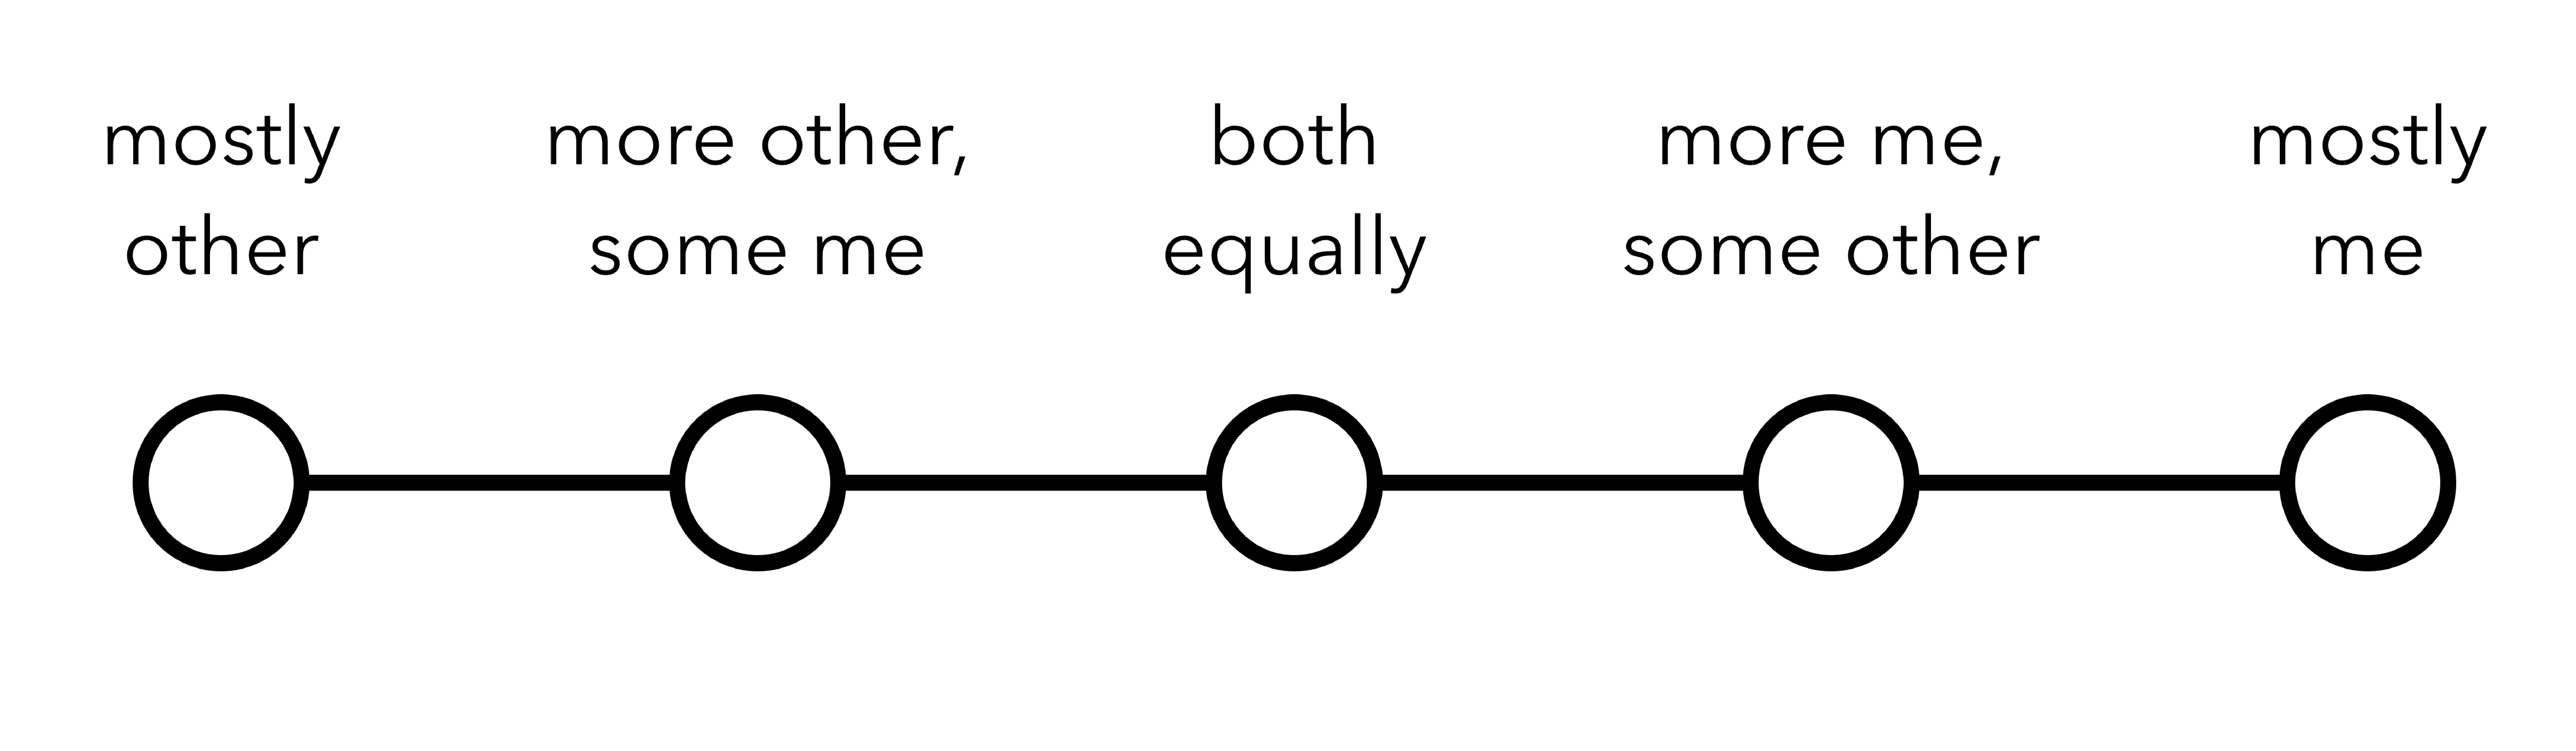
\includegraphics[width=7cm]{likert_scales/ls_5p-team}} \\
\end{tabular}


\noindent\makebox[\linewidth]{\rule{\columnwidth}{0.4pt}}

\noindent
\textbf{[NC] Negotiation and Communication}: Verbal conversation (i.e., talk) facilitated through the ability of utilizing nonverbal information cues in order to discuss and interpret any task-related aspects of the activity (e.g., findings in the data, roles and structure of task approach, and so on).

\noindent
\begin{tabular}{p{1cm}p{9cm}p{8cm}}
NC.1 & According to your impression, how often did you communicate \emph{verbally} to your partner?
    & \raisebox{-.5\height}{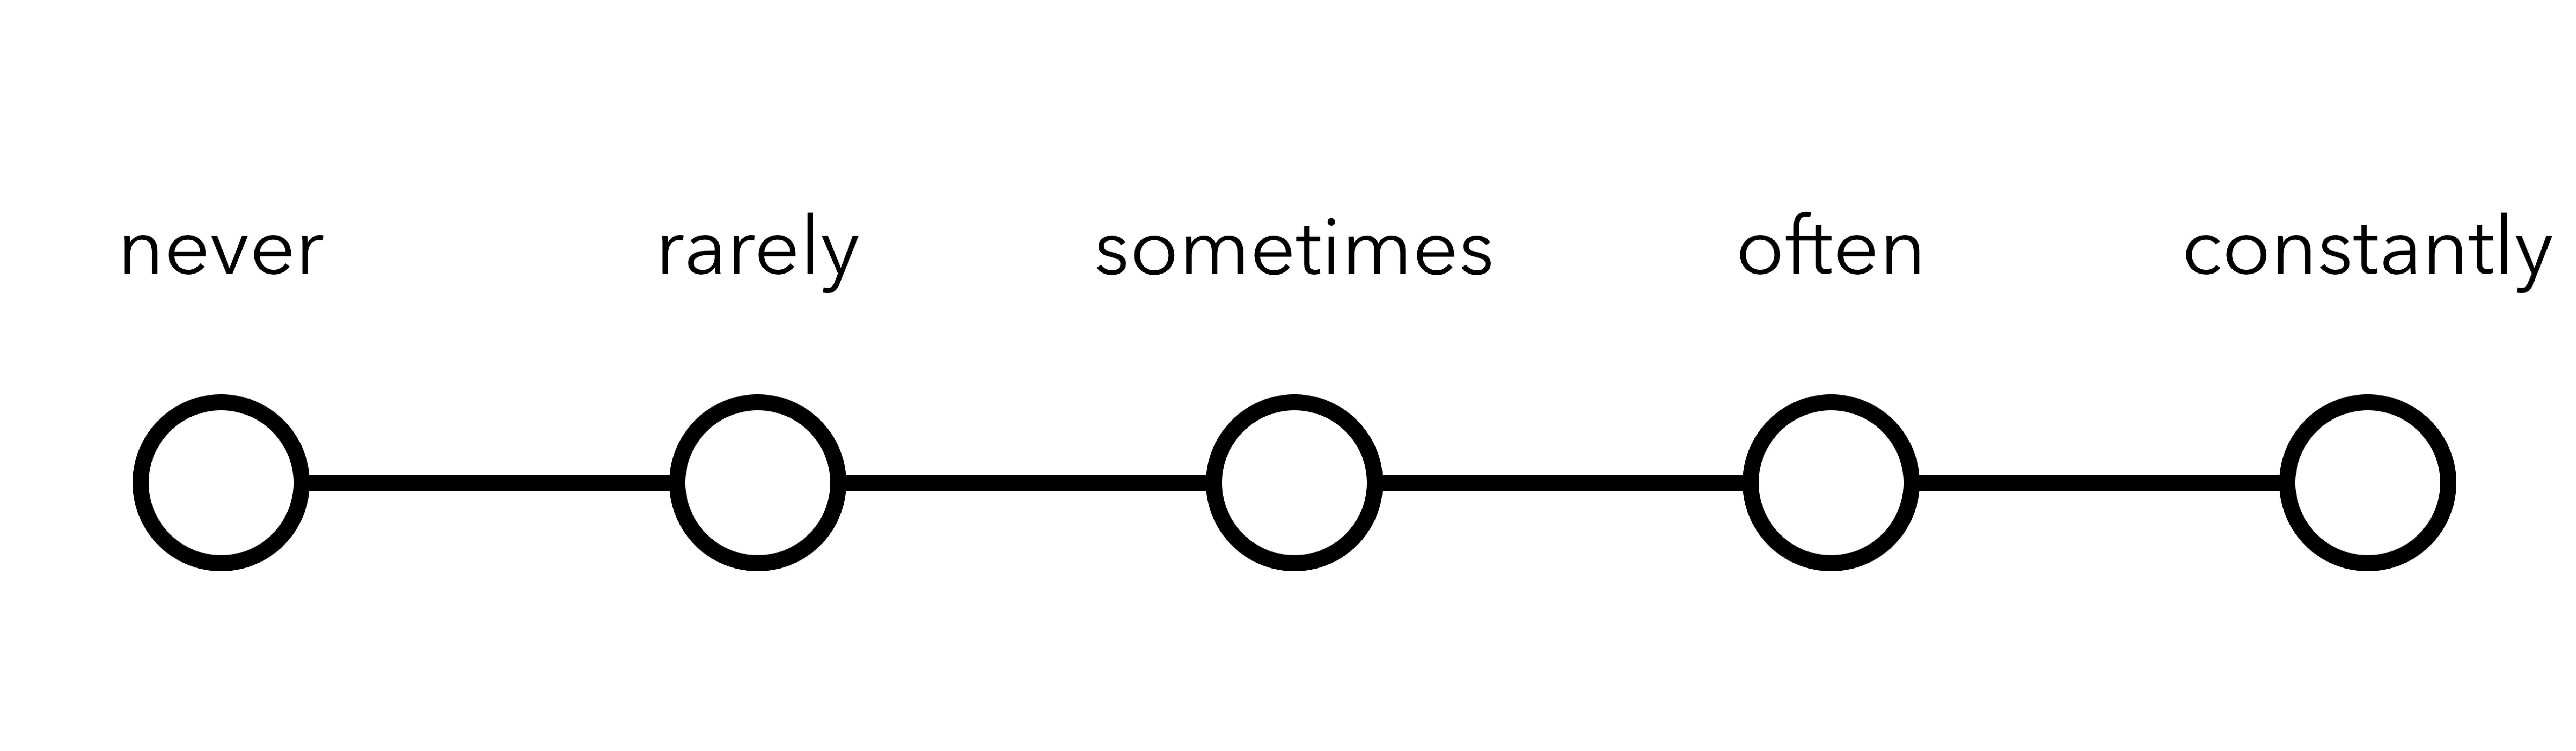
\includegraphics[width=7cm]{likert_scales/ls_5p-never_constantly}} \\
NC.2 & According to your impression, how often did you communicate \emph{nonverbally} to your partner?
    & \raisebox{-.5\height}{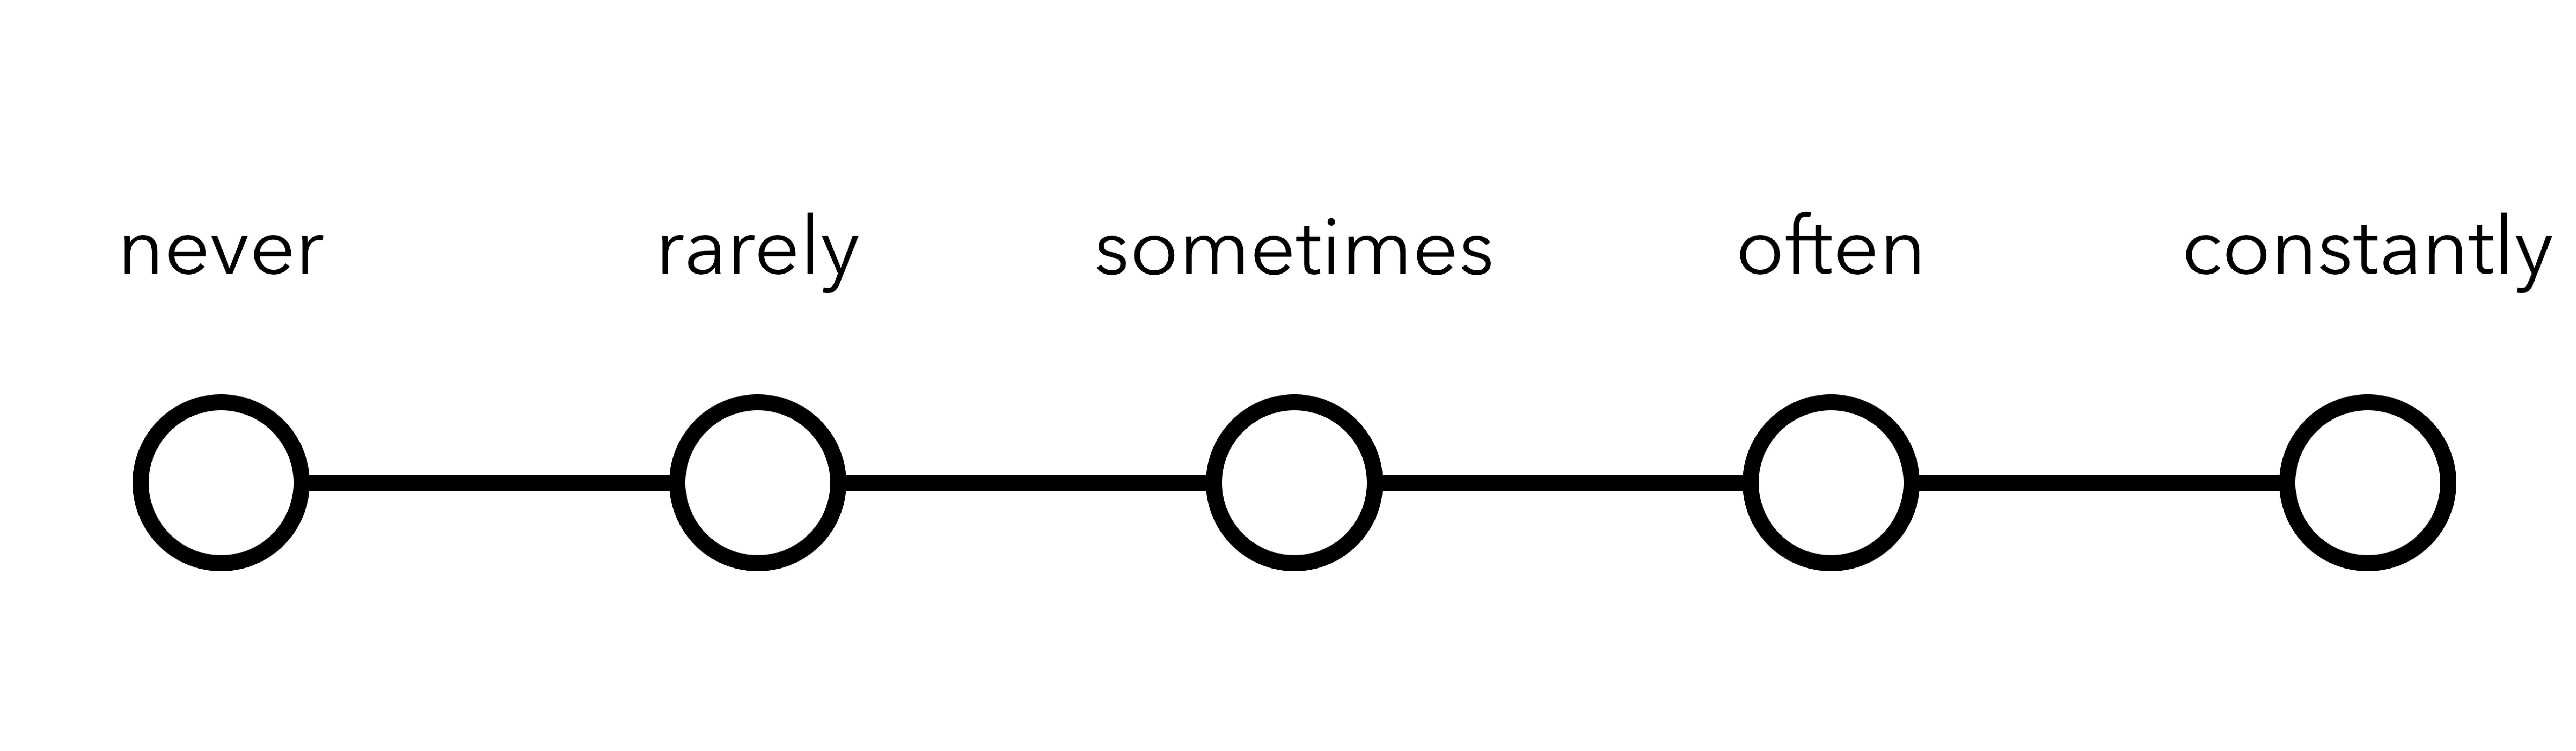
\includegraphics[width=7cm]{likert_scales/ls_5p-never_constantly}} \\
NC.3 & How often would you consider did \emph{dialog} take place?
    & \raisebox{-.5\height}{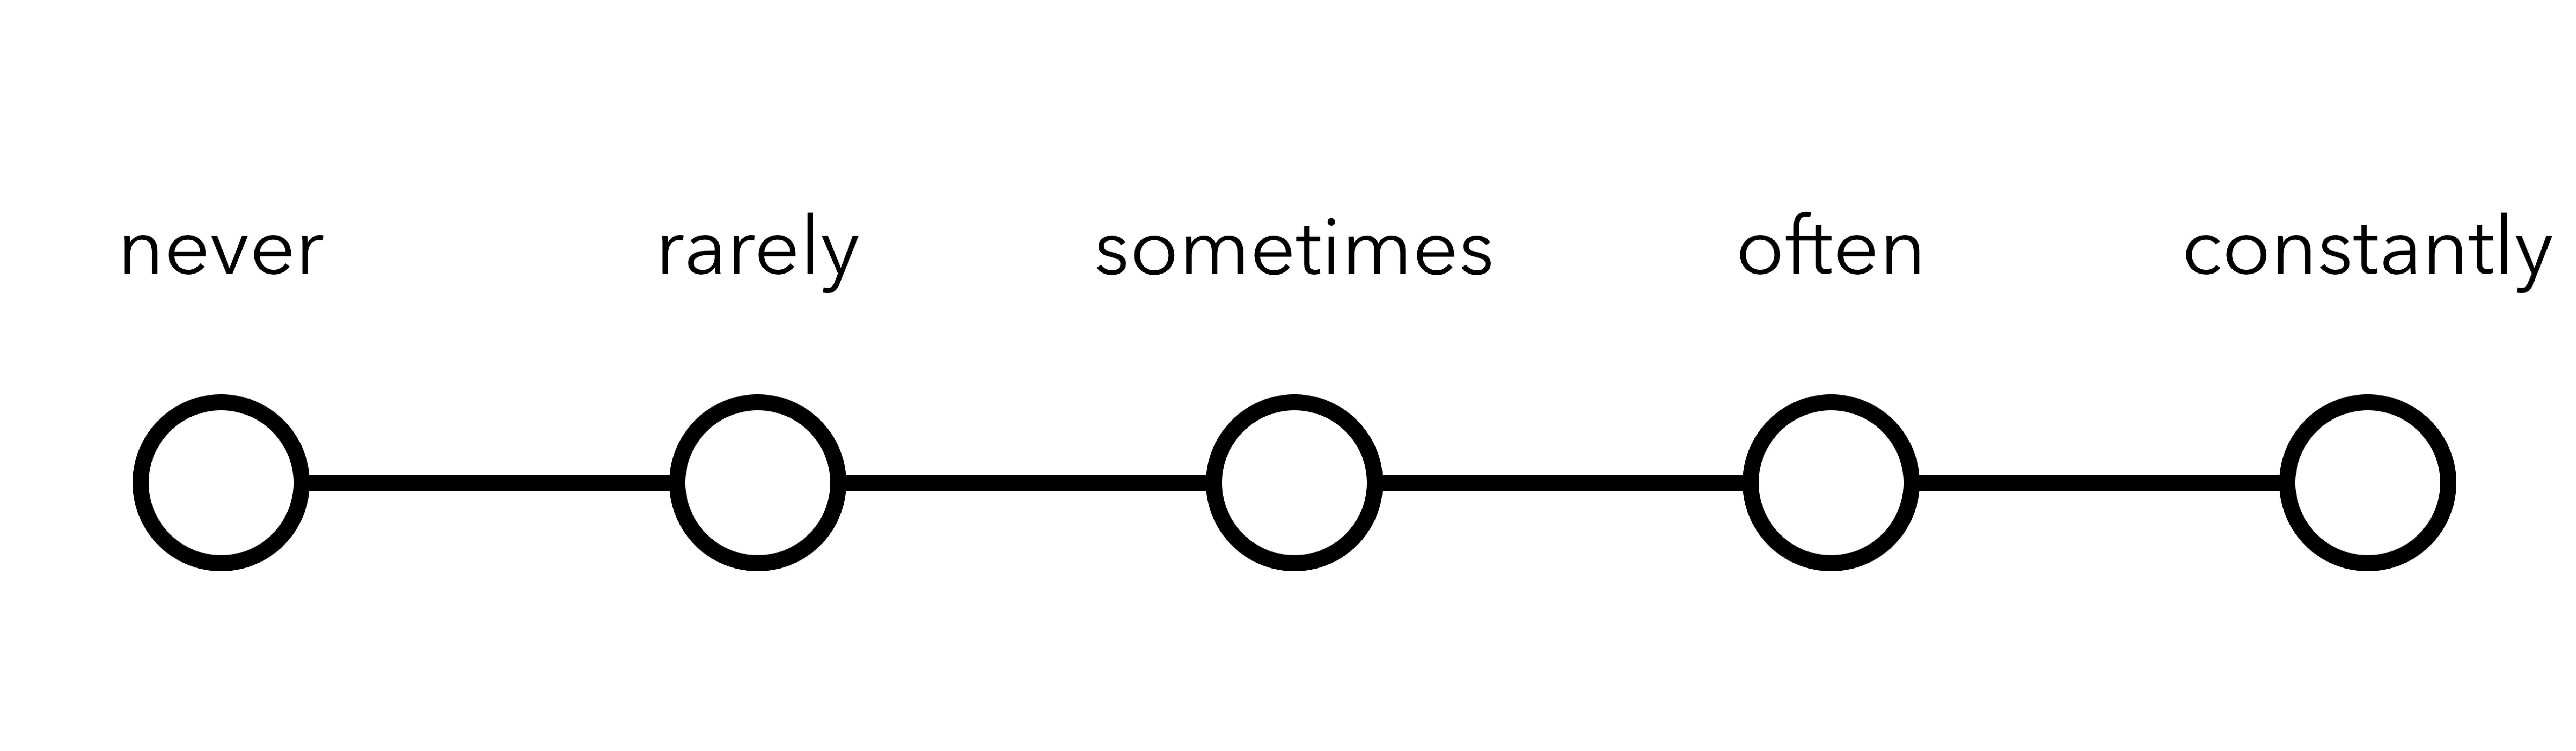
\includegraphics[width=7cm]{likert_scales/ls_5p-never_constantly}} \\
NC.4 & How often would you consider did \emph{negotiation} take place?
    & \raisebox{-.5\height}{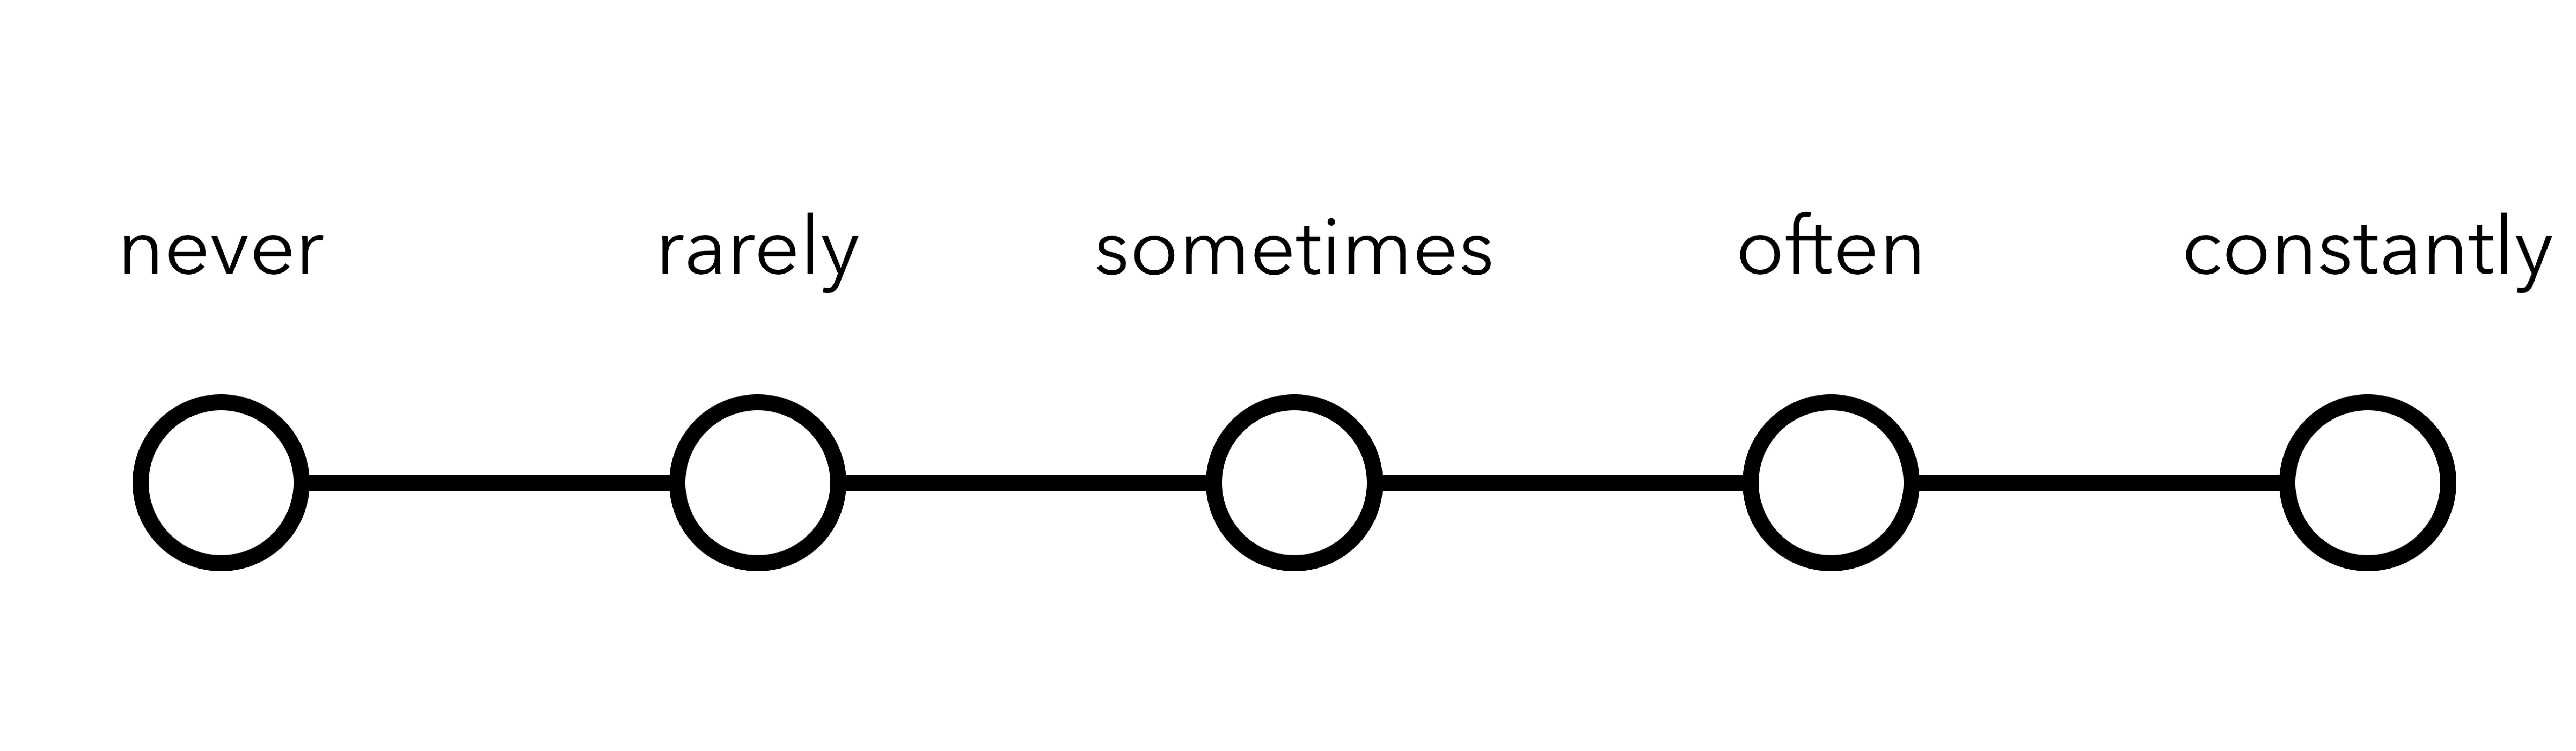
\includegraphics[width=7cm]{likert_scales/ls_5p-never_constantly}} \\
NC.5 & Who would you say mostly initiated the \emph{negotiations}?
    & \raisebox{-.5\height}{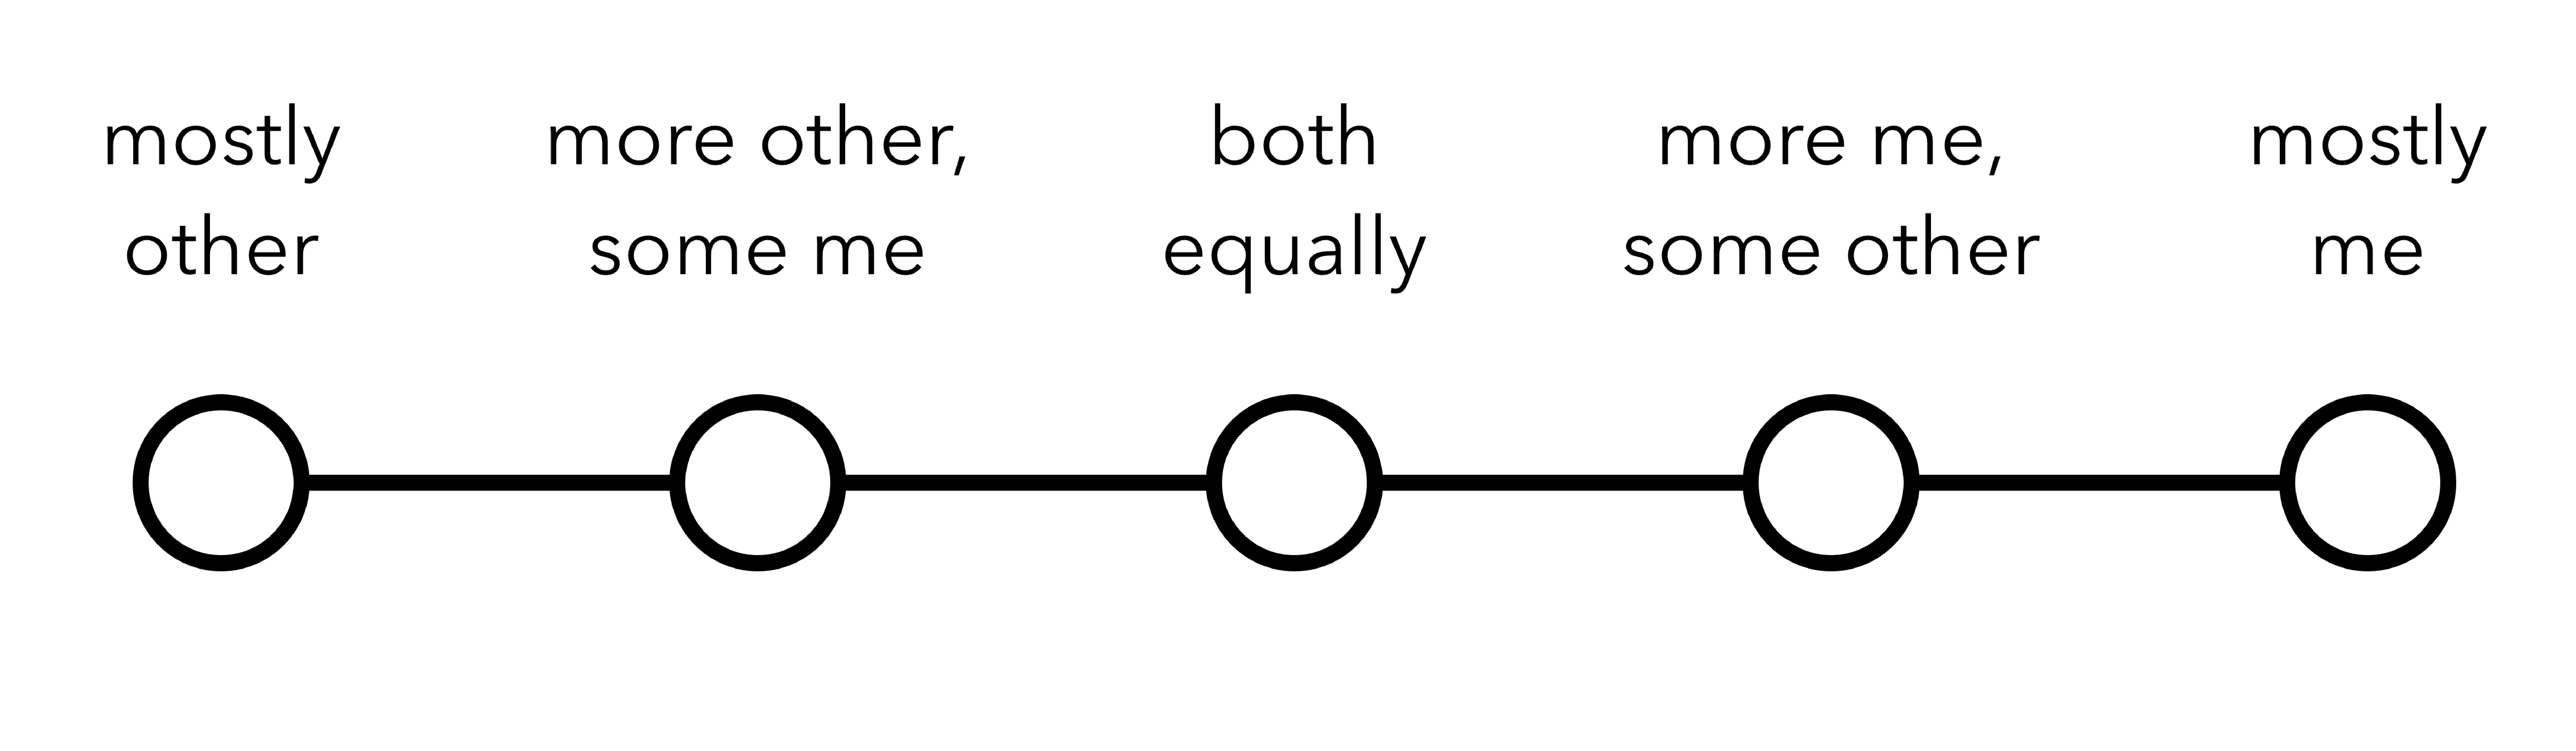
\includegraphics[width=7cm]{likert_scales/ls_5p-team}} \\
\end{tabular}


\noindent\makebox[\linewidth]{\rule{\columnwidth}{0.4pt}}
\emph{Please continue on the next page.}


% === QUESTIONNAIRE DIMENSIONS / ITEMS (PAGE 2) ===
\newpage

\vspace*{2\baselineskip}
\noindent\makebox[\linewidth]{\rule{\columnwidth}{0.4pt}}

\noindent
\textbf{[SC] Sharing Context}: Characteristics and features of the shared space that facilitate and support focused and unfocused collaborative work, leading to shared understandings.

\noindent
\begin{tabular}{p{1cm}p{9cm}p{8cm}}
SC.1  & The collaborative features of the system allowed me to focus on the same subject as my partner. 
    & \raisebox{-.5\height}{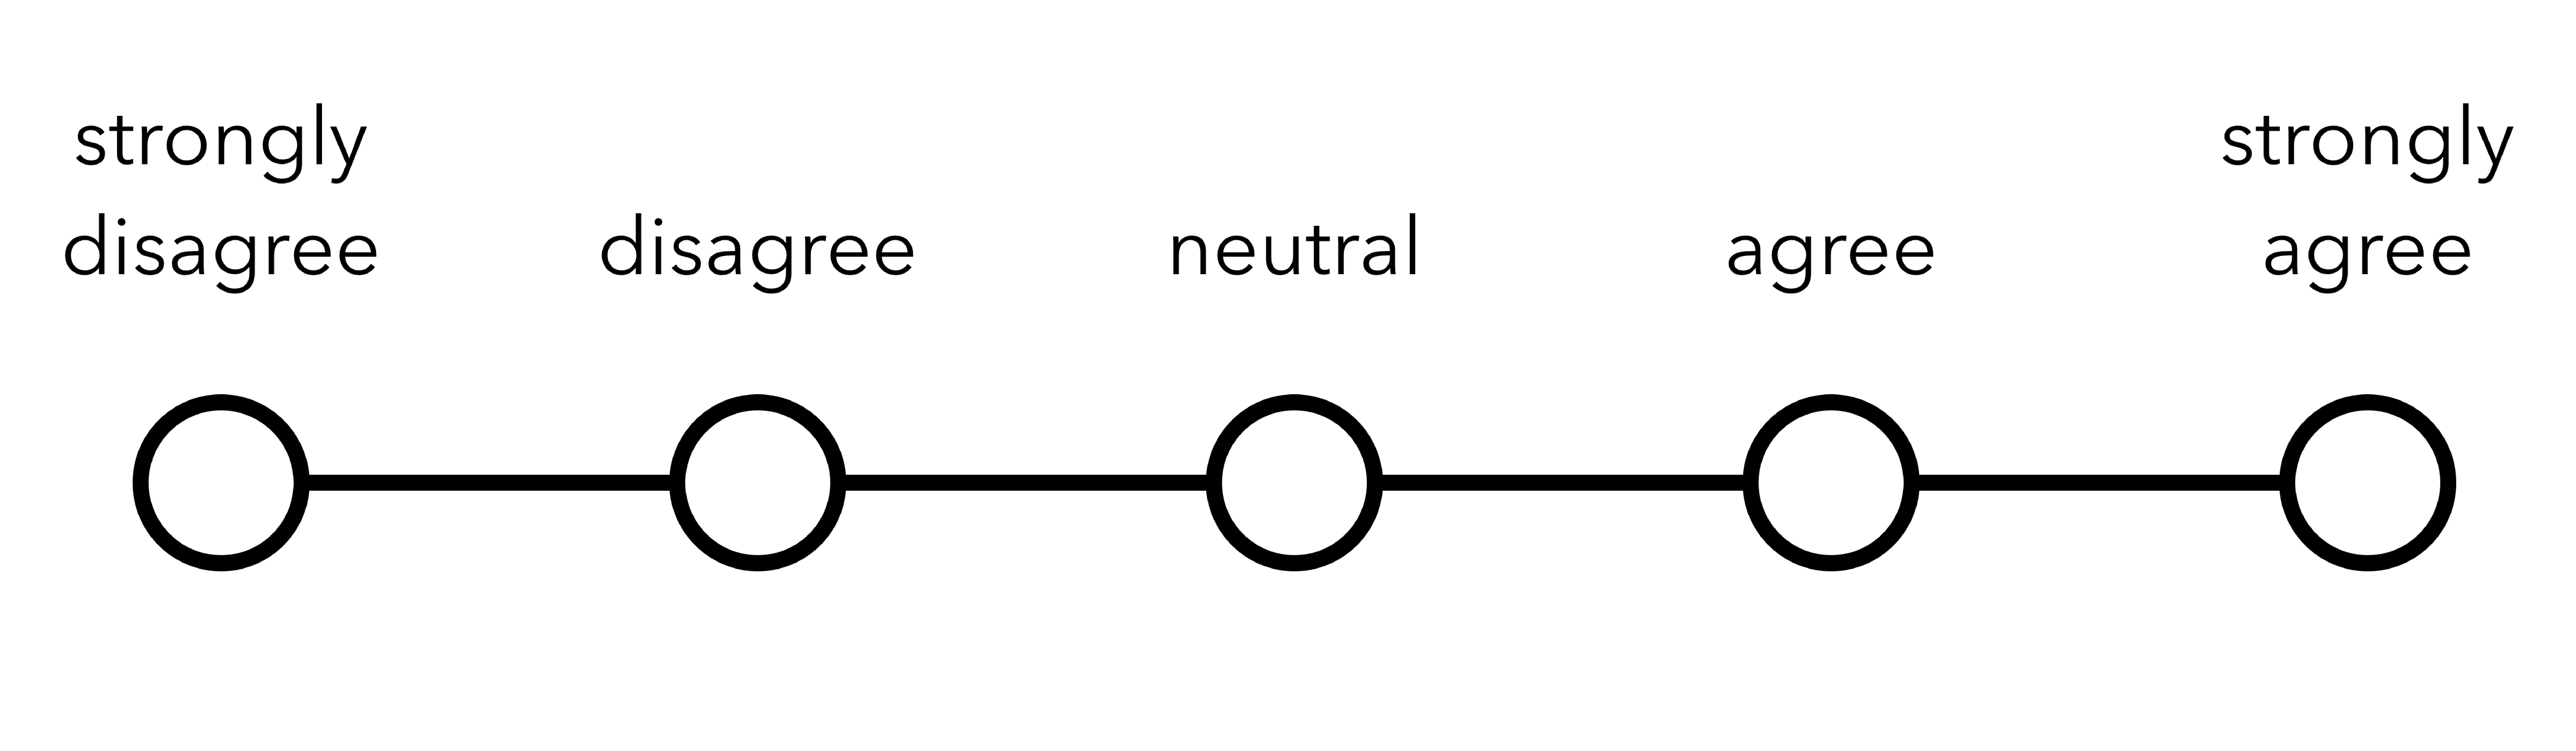
\includegraphics[width=7cm]{likert_scales/ls_5p-agree}} \\
SC.2  & The collaborative features of the system allowed me to establish a dialog with my partner. 
    & \raisebox{-.5\height}{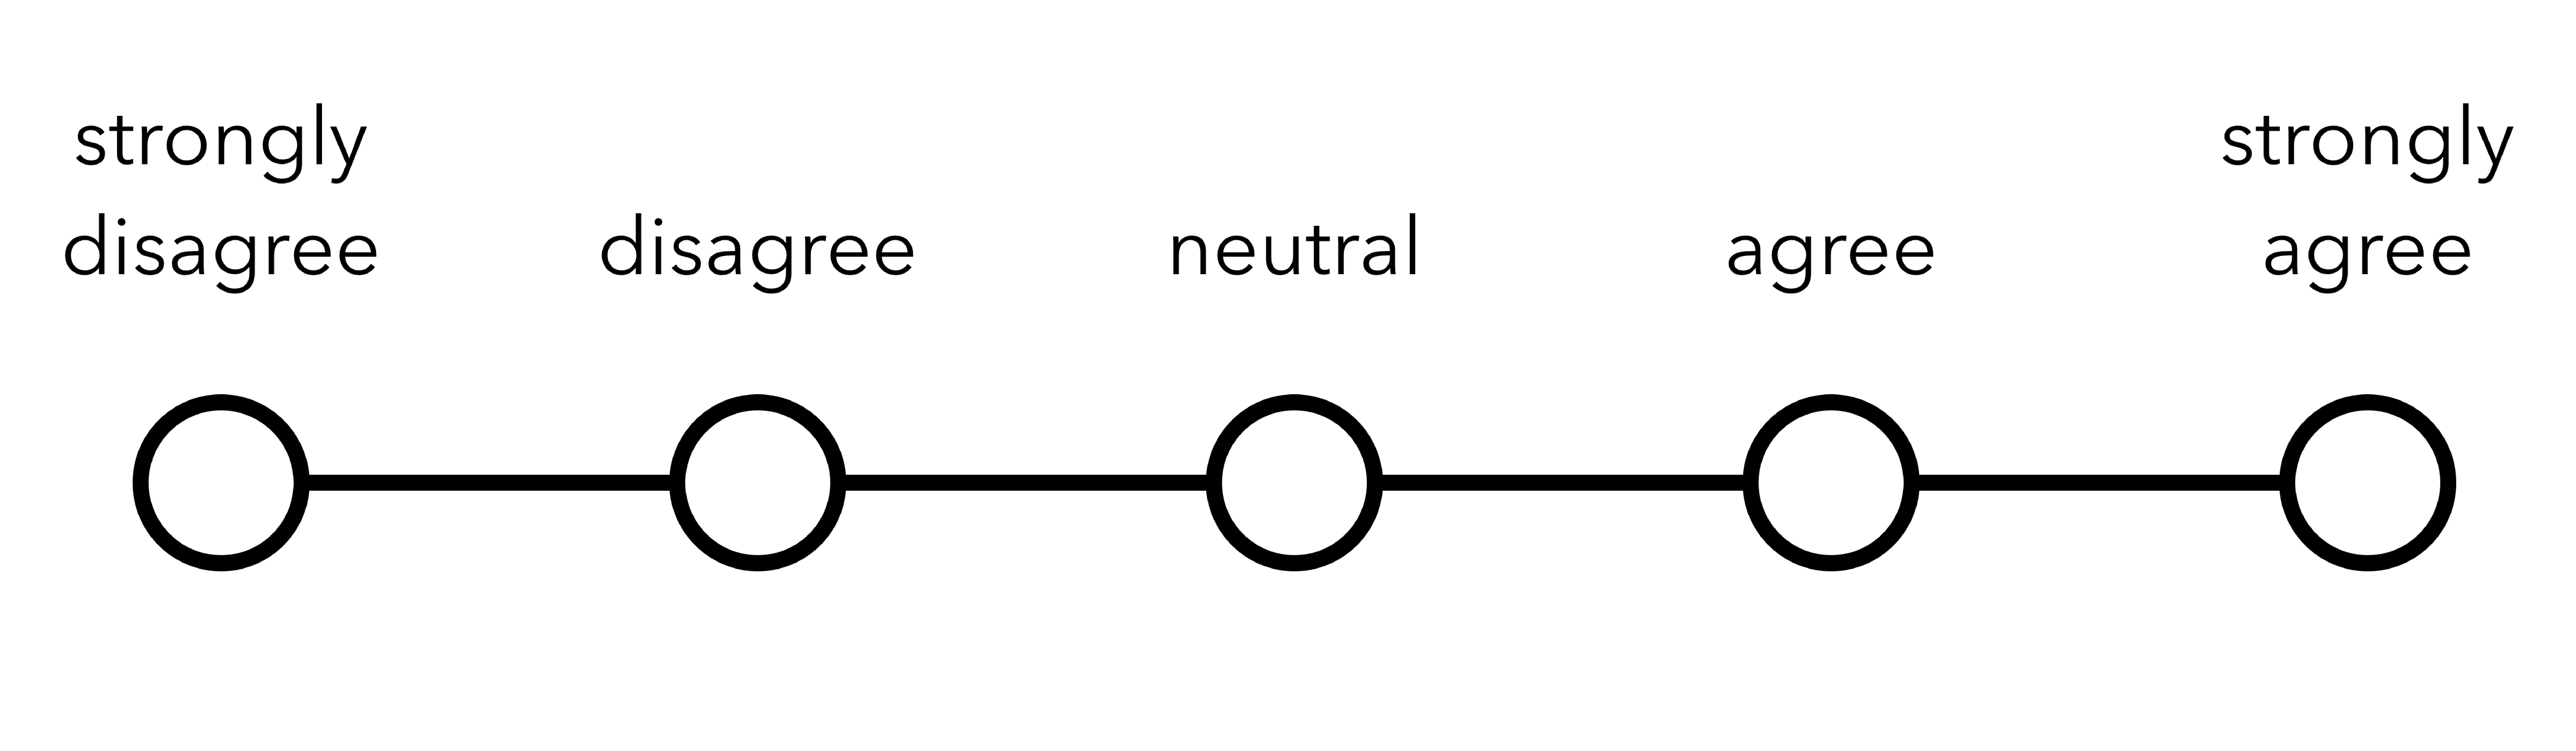
\includegraphics[width=7cm]{likert_scales/ls_5p-agree}} \\
SC.3  & The collaborative features of the system distracted me from my \emph{individual} efforts.
    & \raisebox{-.5\height}{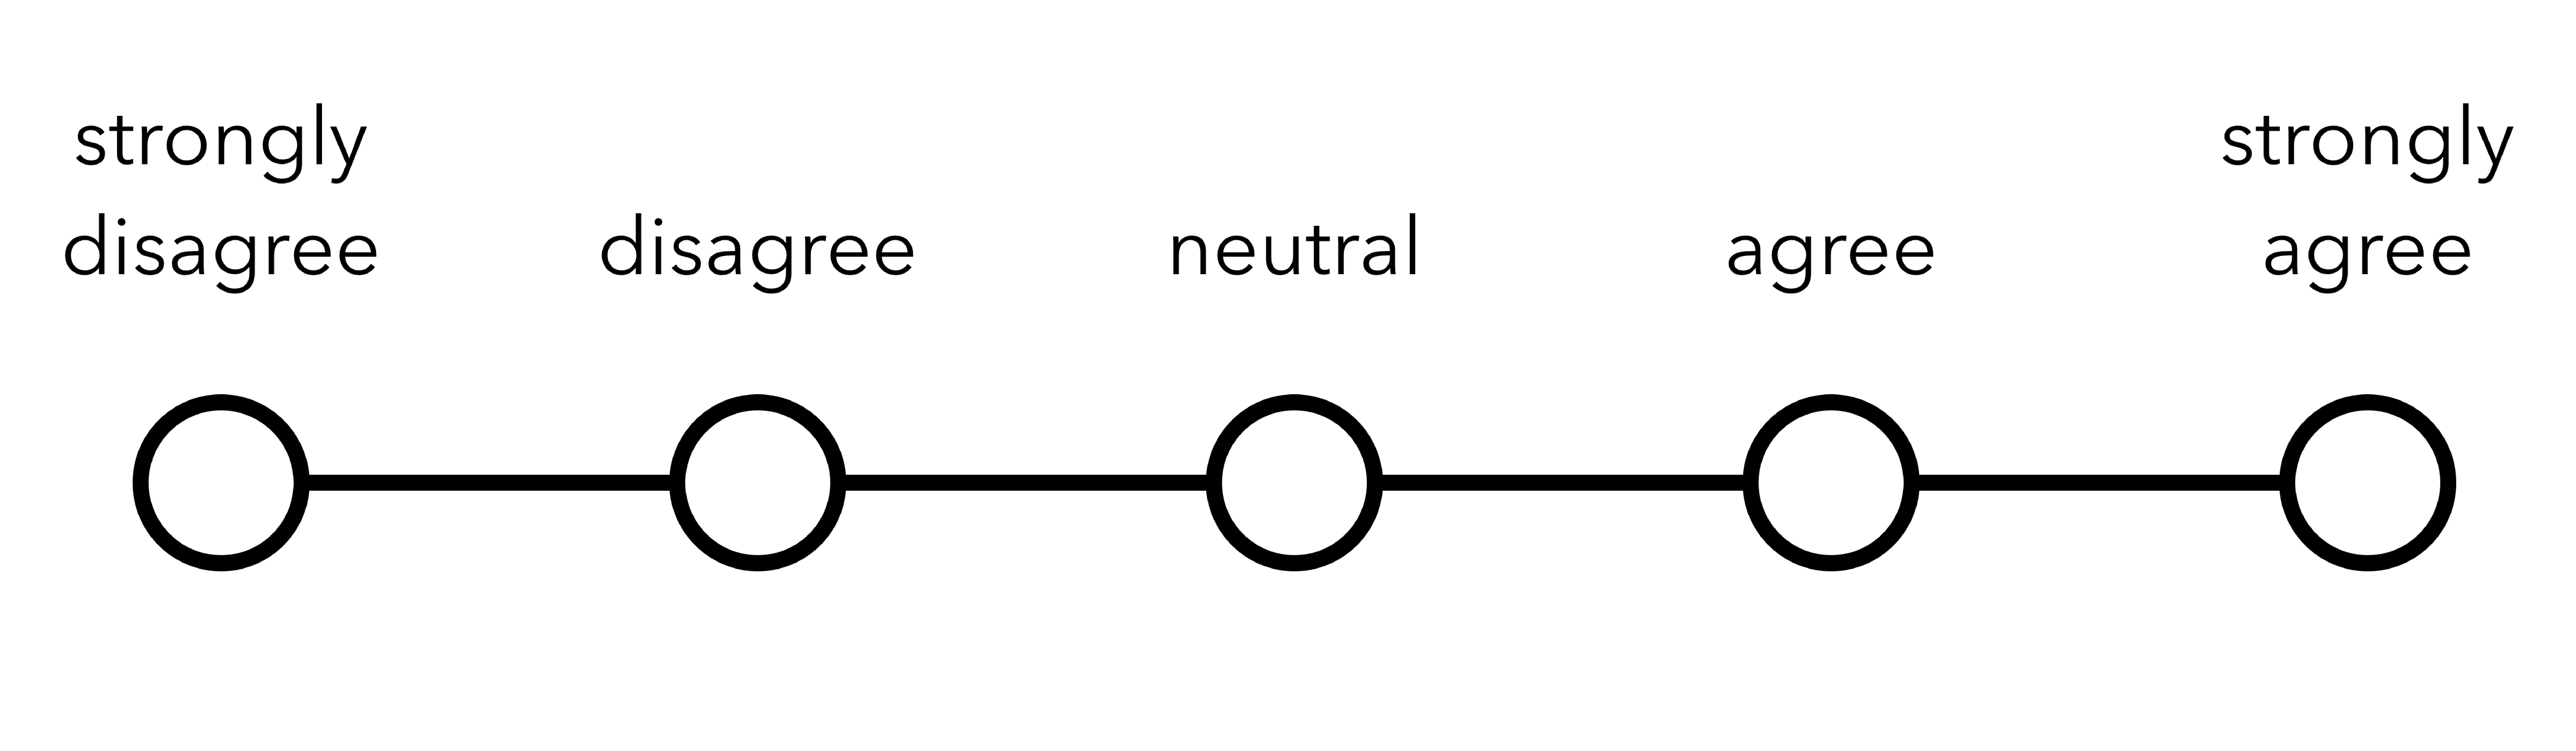
\includegraphics[width=7cm]{likert_scales/ls_5p-agree}} \\
\end{tabular}


\noindent\makebox[\linewidth]{\rule{\columnwidth}{0.4pt}}


\noindent
\textbf{[AO] Awareness of Others}: The ability to understand your partner's activity during times of (1) focused collaboration and active communication (i.e., \emph{group} efforts), as well as (2) more independent and \emph{individual} work.


\noindent
\begin{tabular}{p{1cm}p{9cm}p{8cm}}
AO.1 & During your \emph{group} efforts, how much were you aware of your partner's activities?
    & \raisebox{-.5\height}{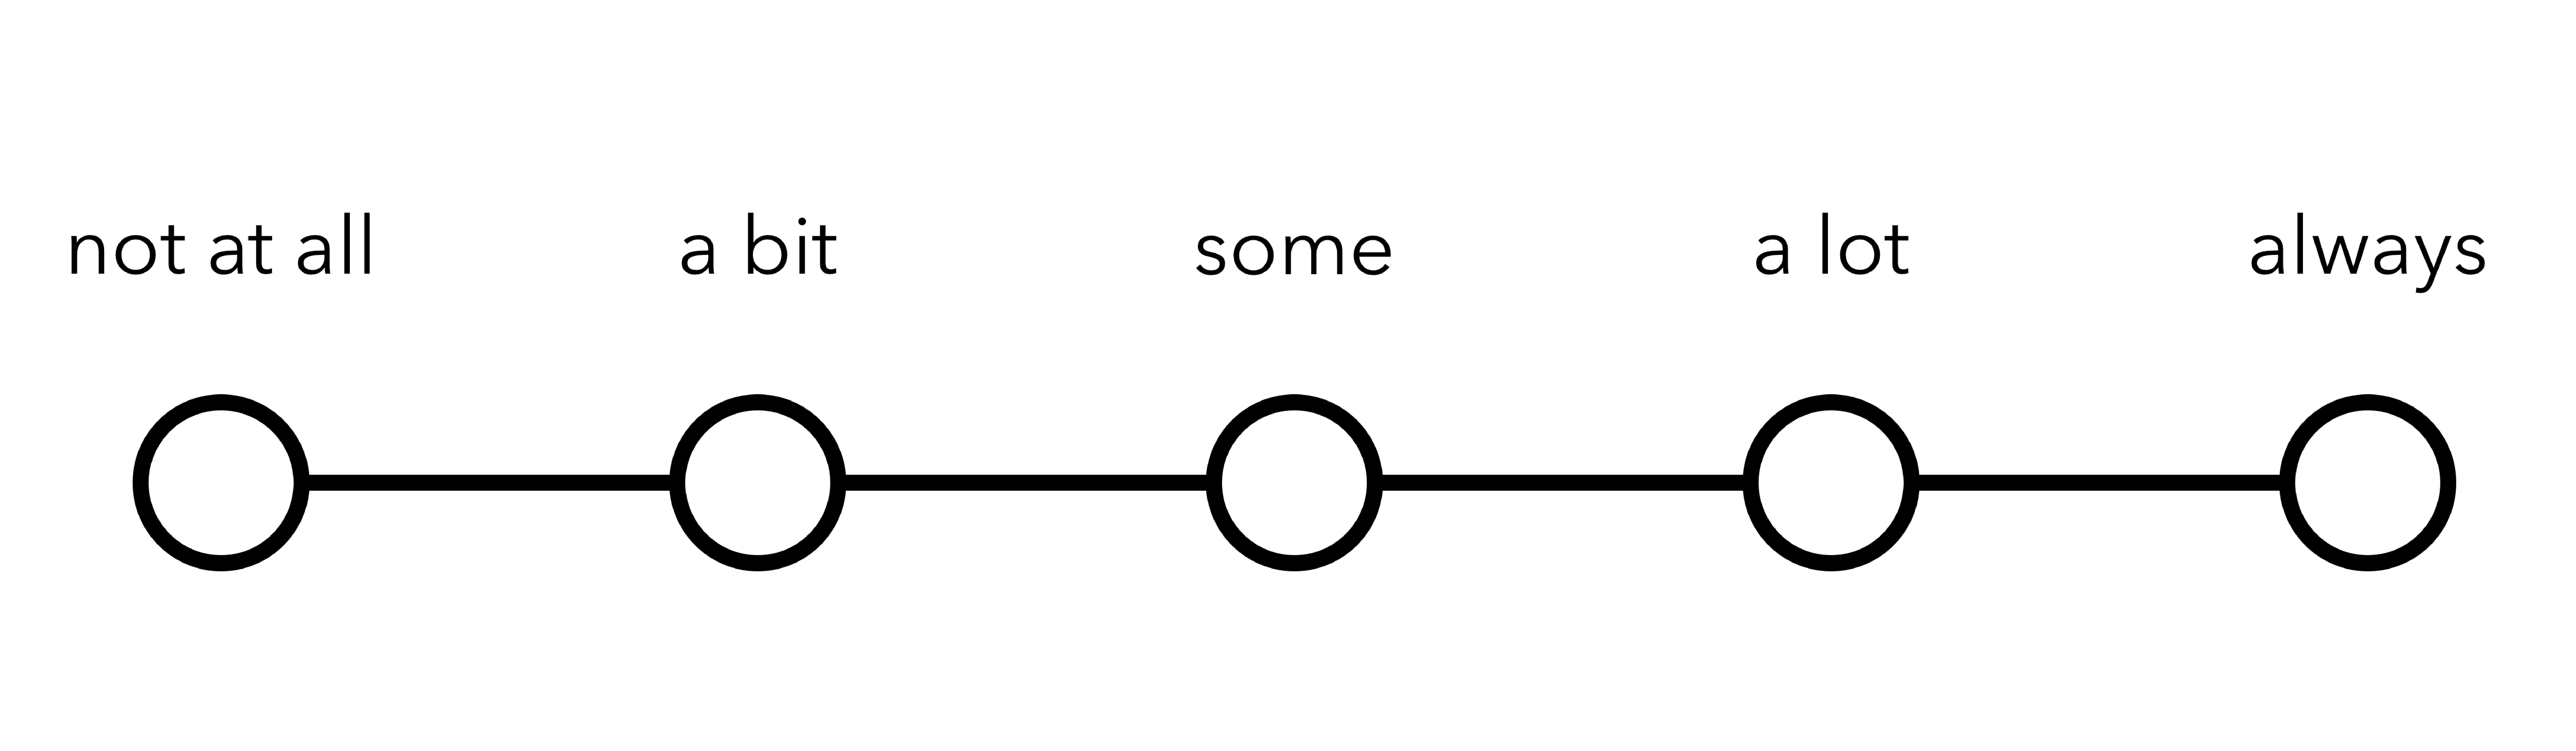
\includegraphics[width=7cm]{likert_scales/ls_5p-not_at_all_always}} \\
AO.2 & During your \emph{group} efforts, how much were you aware of your partner's location in space?
    & \raisebox{-.5\height}{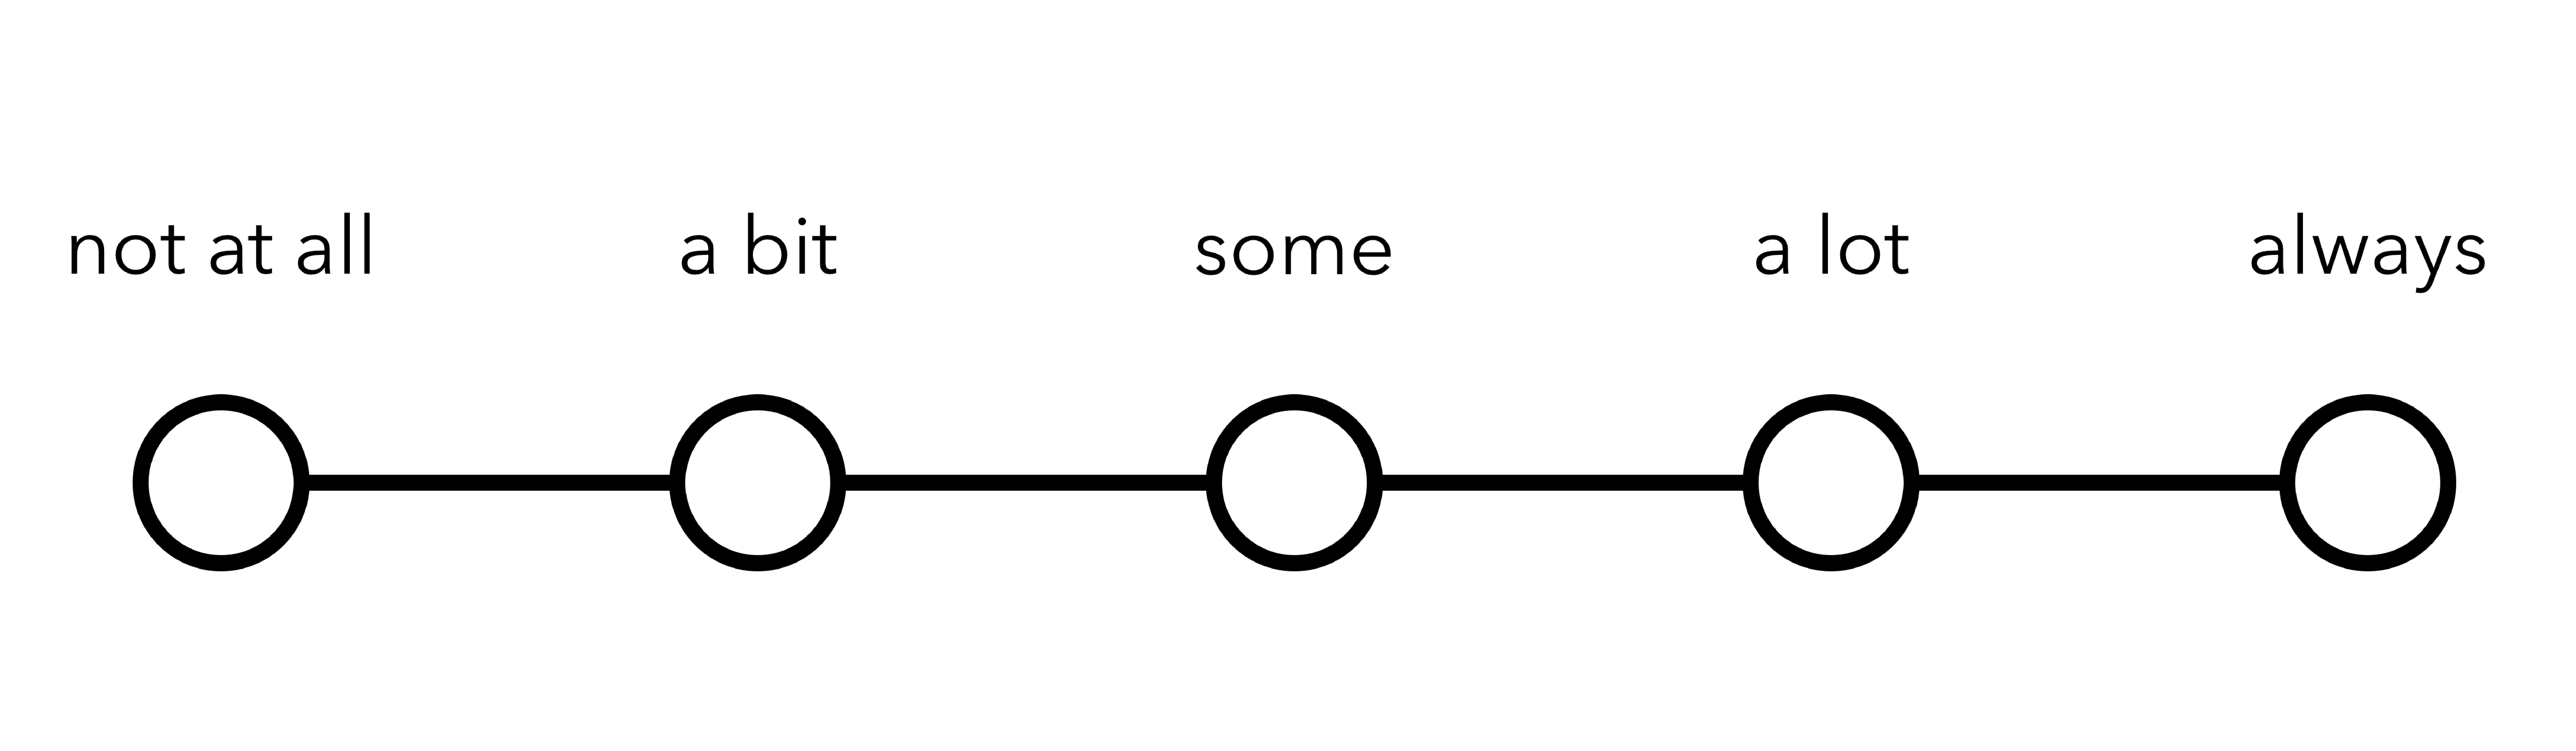
\includegraphics[width=7cm]{likert_scales/ls_5p-not_at_all_always}} \\
AO.3 & During your \emph{group} efforts, how much were you aware of your partner's time reference (time point / interval)?
    & \raisebox{-.5\height}{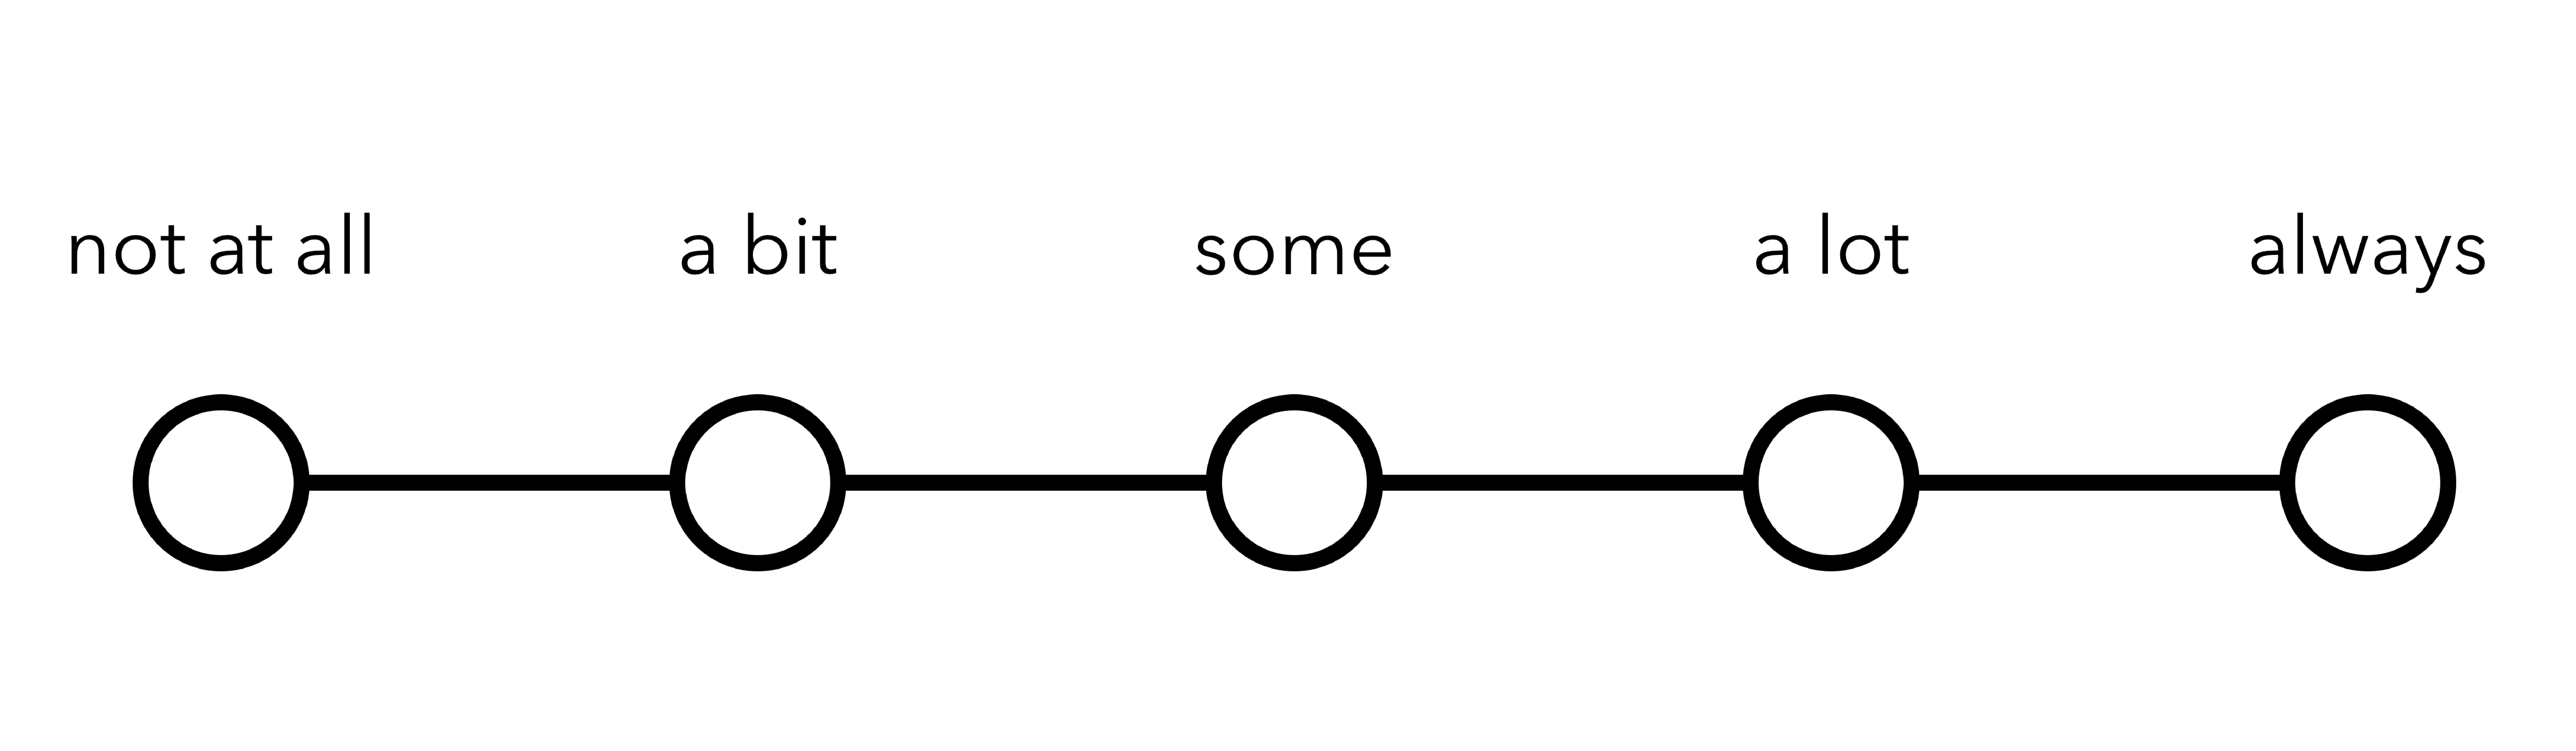
\includegraphics[width=7cm]{likert_scales/ls_5p-not_at_all_always}} \\
AO.4 & During your \emph{individual} efforts, how much were you aware of your partner's activities?
    & \raisebox{-.5\height}{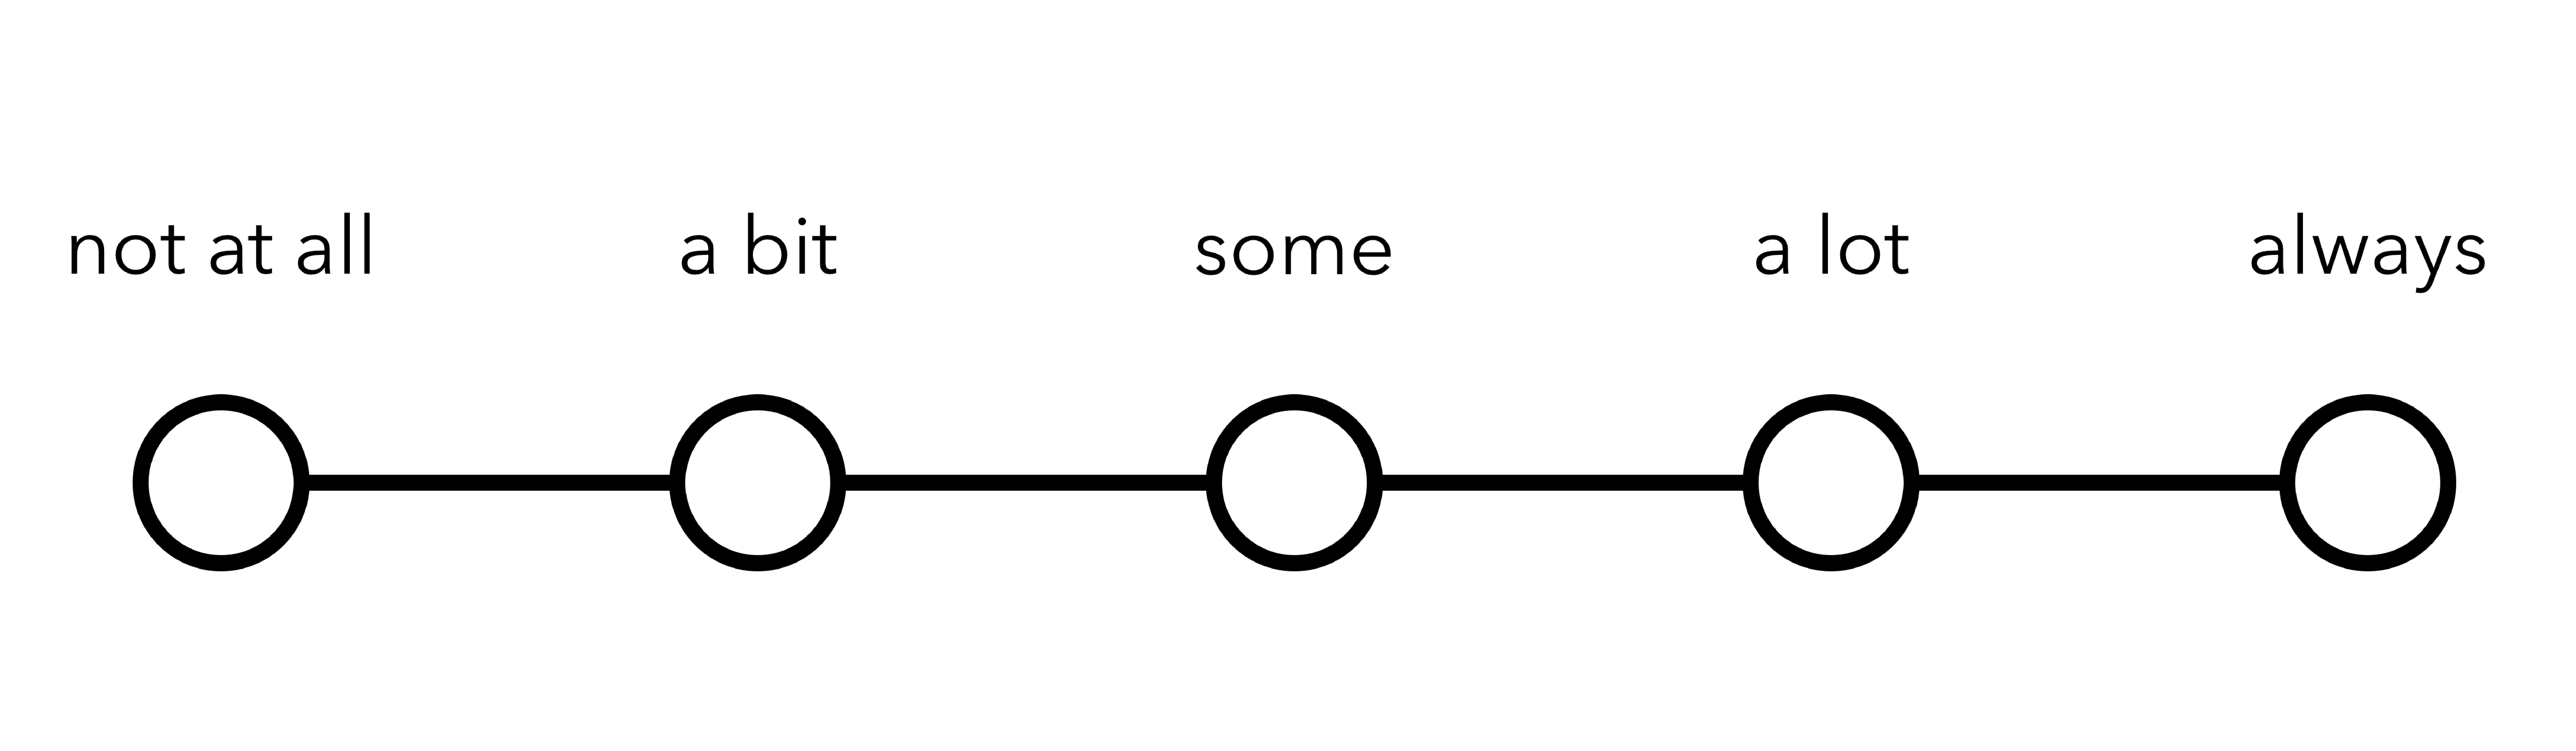
\includegraphics[width=7cm]{likert_scales/ls_5p-not_at_all_always}} \\
AO.5 & During your \emph{individual} efforts, how much were you aware of your partner's location in space?
    & \raisebox{-.5\height}{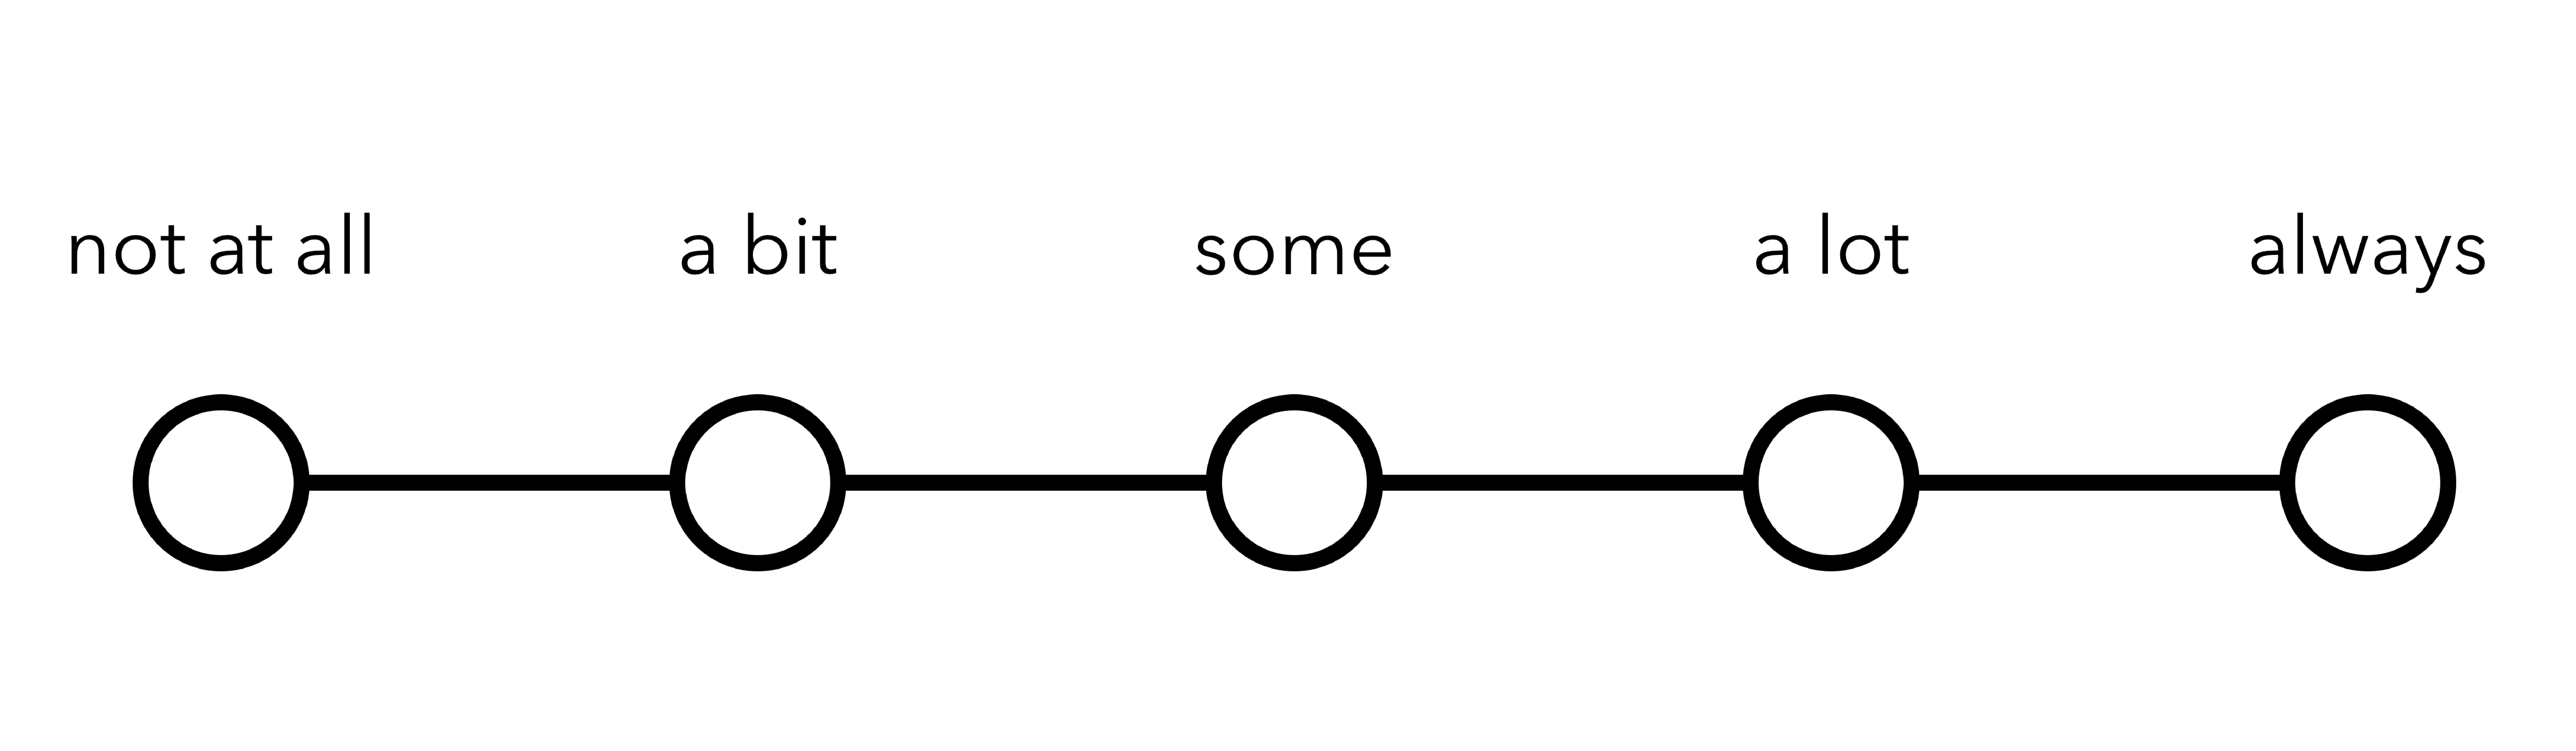
\includegraphics[width=7cm]{likert_scales/ls_5p-not_at_all_always}} \\
AO.6 & During your \emph{individual} efforts, how much were you aware of your partner's time reference (time point / interval)?
    & \raisebox{-.5\height}{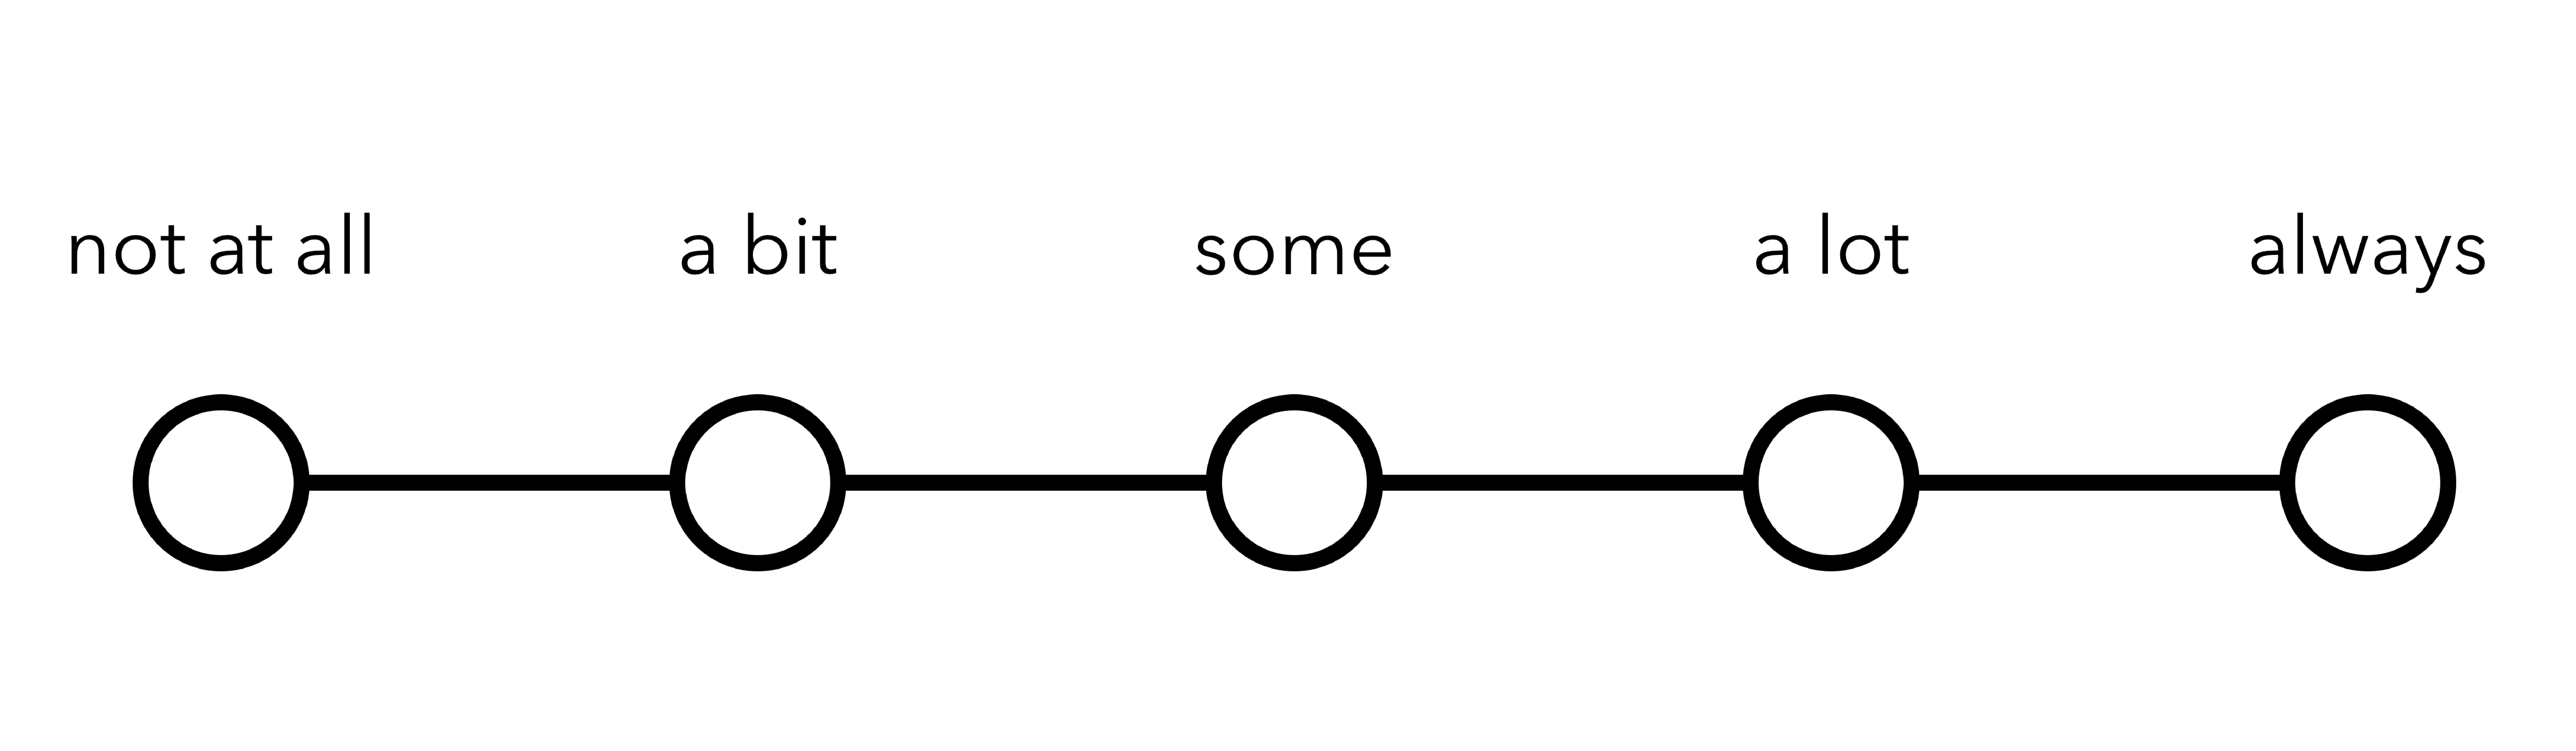
\includegraphics[width=7cm]{likert_scales/ls_5p-not_at_all_always}} \\
\end{tabular}

\noindent\makebox[\linewidth]{\rule{\columnwidth}{0.4pt}}

\end{document}
% === DOCUMENT - END ===